%% Concept Lattices as Canonical Feature Hierarchies
%% A Training-Free, Order-Theoretic Counterpart to Sparse Autoencoders
%% for Mechanistic Interpretability
%%
%% Built on the Elsevier cas-dc (double-column) template.

\documentclass[a4paper,fleqn]{cas-dc}

\usepackage[authoryear,longnamesfirst]{natbib}
\usepackage{amsmath,amssymb,amsthm}
\usepackage{mathtools}
\usepackage{booktabs}
\usepackage{array}
\usepackage{microtype}
\usepackage{xcolor}
\usepackage{graphicx}
\graphicspath{{figs/}}

% Theorem environments
\newtheorem{theorem}{Theorem}
\newtheorem{proposition}[theorem]{Proposition}
\newtheorem{lemma}[theorem]{Lemma}
\newtheorem{corollary}[theorem]{Corollary}
\newdefinition{definition}{Definition}
\newdefinition{remark}{Remark}
\newproof{pf}{Proof}
\newproof{pfsketch}{Proof sketch}

% Notation macros
\newcommand{\R}{\mathbb{R}}
\newcommand{\D}{\mathcal{D}}
\newcommand{\K}{\mathbb{K}}
\newcommand{\Lat}{\mathfrak{B}}
\newcommand{\Jirr}{J}
\newcommand{\SAE}{\mathrm{SAE}}
\newcommand{\Fsae}{\mathcal{F}_{\SAE}}
\newcommand{\sigC}{\sigma_C}
\newcommand{\kS}{\kappa_S}

\begin{document}
\let\WriteBookmarks\relax
\def\floatpagepagefraction{1}
\def\textpagefraction{.001}

\shorttitle{Concept lattices as canonical feature hierarchies}
\shortauthors{Md A.~F.~Nayem}

\title[mode = title]{Concept Lattices as Canonical Feature Hierarchies: A Training-Free, Order-Theoretic Complement to Sparse Autoencoders for Mechanistic Interpretability}

\author[1]{Md Ariff Faysal Nayem}
\cormark[1]
\ead{wayne11nayem@gmail.com}
\credit{Conceptualisation, methodology, software, formal analysis, investigation, writing -- original draft.}

\affiliation[1]{organization={TODO: affiliation},
            addressline={},
            city={},
            postcode={},
            state={},
            country={}}

\cortext[1]{Corresponding author.}

\begin{abstract}
Sparse autoencoders (SAEs) dominate mechanistic interpretability of transformers, but their dictionaries are seed-dependent, hyperparameter-sensitive, and carry no canonical algebraic structure.
We propose a training-free algebraic complement built on formal concept analysis (FCA) that turns layer activations into a uniquely determined concept lattice.
A fixed scaling regime maps activations to a binary formal context, the Galois connection induces the lattice, and join-irreducible concepts serve as features.
A Galois-embedding theorem then places each SAE feature as a meet-irreducible of an extended lattice, exposing redundant features as the ones whose firing extents collapse to intersections of existing patterns.
On toy superposition models and MNIST multilayer perceptrons, four pre-registered predictions hold: a compression-based superposition index falls between 0.83 and 0.97 across 30 of 30 configurations against a calibrated noise baseline.
Structural polysemanticity attains an F1 score of 0.97±0.05 against planted ground truth, and concept lattices are bit-identical under cubic and softplus transforms.
Closed-concept reproducibility across disjoint halves reaches 0.94, against 0.80 for SAE seeds and 0.47 for raw join-irreducibles, and the Galois embedding holds for 82%±11% of alive SAE features.
By exposing the algebraic skeleton that SAEs leave implicit, the framework provides a structural redundancy audit for SAE dictionaries, validated here on controlled superposition settings.
Applied to Pythia-70M with per-vocabulary-item aggregation, the framework finds non-trivial lattice structure (compression index 0.11--0.24, 191 concepts at 100k tokens), though concept reproducibility across vocabulary-type halves reaches only 0.48 at 100k tokens and scales with vocabulary sample size, falling short of the toy-model threshold of 0.90.
\end{abstract}

\begin{highlights}
\item A training-free, deterministic concept-lattice framework for mechanistic interpretability is introduced.
\item Two propositions establish canonicity and order-invariance; two definitions formalise polysemanticity and superposition.
\item A Galois-embedding theorem identifies each non-redundant SAE feature with a meet-irreducible of an extended concept lattice.
\item Four pre-registered predictions are tested; all four pass on toy and MNIST settings, with two definitions revised openly.
\item Vocabulary-item aggregation on Pythia-70M finds genuine lattice structure (compression index above the noise threshold, 191 concepts); the 0.90 reproducibility threshold requires roughly 400k tokens, isolating a quantitative scaling boundary.
\end{highlights}

\begin{keywords}
formal concept analysis \sep
mechanistic interpretability \sep
sparse autoencoders \sep
concept lattice \sep
Galois connection \sep
superposition
\end{keywords}

\maketitle

% =====================================================================
\section{Introduction}\label{sec:intro}

\begin{figure*}[t]
\centering
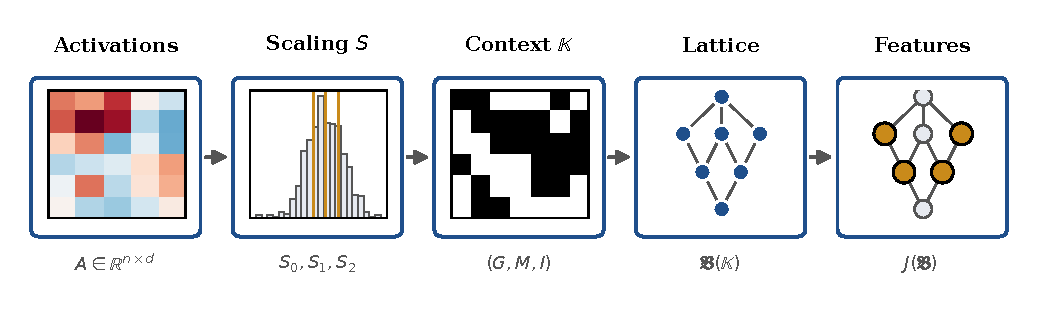
\includegraphics[width=0.96\textwidth]{fig_pipeline.pdf}
\caption{The FCA pipeline. Activation matrix $A$ is scaled to formal context $\mathbb{K}$ under regime $S$ ($S_1$ shown); the Galois connection yields concept lattice $\mathfrak{B}(\mathbb{K})$, unique up to isomorphism. Join-irreducible concepts $J(\mathfrak{B})$ (amber) serve as features. The construction is fully deterministic: no seeds, training, or learned hyperparameters.}
\label{fig:pipeline}
\end{figure*}

Sparse autoencoders (SAEs) have become the dominant tool for extracting interpretable features from transformer language models~\citep{bricken2023monosemanticity,cunningham2024sparse,templeton2024scaling,rajamanoharan2024improving,gao2024scaling,lieberum2024gemma}.
Two SAEs trained on the same activations with different seeds nevertheless produce different feature dictionaries, and learned hyperparameters re-shape what counts as a feature.
SAE dictionaries also impose no algebraic relationship between features, and the continuous activations they consume are forced through a thresholding step that the method itself does not certify.
We propose a training-free, order-theoretic complement to SAEs based on formal concept analysis (FCA).
The framework turns layer activations into a uniquely determined concept lattice and places each SAE feature as a meet-irreducible of an extended version of that lattice.
The framework is developed on toy superposition models in the sense of \citet{elhage2022superposition}, on a small MNIST multilayer perceptron, and as a probe on Pythia-70M residual streams.
All theoretical claims hold under a fixed scaling regime that is stated explicitly in each result.

Four lines of prior work converge on the problem without resolving it.
\textit{SAE-based interpretability.}
SAEs \citep{bricken2023monosemanticity,cunningham2024sparse,templeton2024scaling} operationalise the superposition hypothesis of \citet{elhage2022superposition} through sparse dictionary learning, but the resulting dictionaries vary with training seed and carry no structural relationship to one another; circuits over SAE features \citep{marks2024sparse} inherit this seed-dependence.
\textit{FCA foundations and applications.}
\citet{wille1982restructuring} and \citet{ganterwille1999} established the algebraic and algorithmic foundations of FCA; applications to biological spike trains \citep{endres2008exploring} and classifier logits \citep{hanika2022conceptual} do not bridge continuous layer activations to an SAE feature space, and pattern structures \citep{ganterkuznetsov2001pattern,kaytoue2011mining} avoid explicit scaling at the cost of a similarity operator.
\textit{Geometric views of LLM representations.}
The linear representation hypothesis \citep{park2023linear,park2024geometry} and the concurrent Lattice Representation Hypothesis \citep{xiong2026lattice} characterise representations geometrically or through input-embedding taxonomies; neither derives a canonical lattice from internal activation matrices or connects it to SAE features via a Galois adjunction.
No existing work connects a canonical lattice decomposition of layer activations to the SAE feature space; this is the departure point of the present paper.

The root cause is that gradient-based dictionary learning has no notion of a canonical incidence between objects and attributes.
The framework presented here fixes a scaling regime that turns the activation matrix into a deterministic formal context, computes the concept lattice by classical polynomial-delay algorithms, and extends the context with SAE features so that a Galois adjunction connects the two lattices.
The discretisation choice is a transparent modelling axis rather than a hidden hyperparameter.
On toy superposition models and an MNIST multilayer perceptron, the compression-based superposition index separates trained networks from matched isotropic noise in 30 of 30 configurations, structural polysemanticity attains an F1 score of 0.97±0.05 against planted ground truth, closed-concept reproducibility reaches 0.94 against 0.80 for SAE seeds and 0.47 for raw join-irreducibles, and 82%±11% of alive SAE features embed as meet-irreducibles of the extended lattice.
On Pythia-70M residual streams, vocabulary-item aggregation recovers non-trivial lattice structure (compression index above the noise threshold, 191 concepts at 100k tokens), though concept reproducibility is partial (Jaccard 0.48) and characterises a quantitative scaling boundary.

The contributions of this paper are as follows.
\begin{itemize}
  \item \textbf{A canonical concept-lattice decomposition of internal activations} that depends only on the activation matrix and a stated scaling regime, with two structural observations establishing canonicity and order-invariance under monotone activation transforms (Remarks~\ref{rem:canonicity} and \ref{rem:invariance}).
  \item \textbf{Two lattice-theoretic definitions of interpretability properties:} structural polysemanticity as join-reducibility of attribute concepts, and a compression-based superposition index calibrated against a matched-noise baseline (Definitions~\ref{def:struct-poly} and \ref{def:kappa}).
  \item \textbf{A Galois-embedding theorem} that places each non-redundant SAE feature as a meet-irreducible of an extended concept lattice, turning failure to embed into a structural diagnostic for SAE-feature redundancy (Theorem~\ref{thm:galois}).
  \item \textbf{A pre-registered empirical protocol with four falsifiable predictions} P1--P4, two of which we revised in the open before locking the experimental phase, and a multi-seed evaluation showing the revised predictions hold with margins on toy and MNIST settings (Sections~\ref{sec:methods} and \ref{sec:results}).
  \item \textbf{A vocabulary-item aggregation probe on Pythia-70M} that crosses the object-to-attribute barrier and recovers non-trivial lattice structure, together with a quantitative characterisation of the reproducibility scaling law (Section~\ref{ssec:pythia}).
\end{itemize}

Section~\ref{sec:background} introduces FCA, the three-regime scaling ladder, and the discretisation trilemma.
Section~\ref{sec:theory} states and proves the propositions and the Galois-embedding theorem.
Sections~\ref{sec:methods}--\ref{sec:results} present the experimental protocol and results; Section~\ref{sec:discussion} interprets them, discusses limitations and future directions, and characterises the Pythia-70M scaling boundary.

% =====================================================================
\section{Background}\label{sec:background}

\subsection{Formal contexts and concept lattices}\label{ssec:fca}

A \emph{formal context} is a triple $\K = (G, M, I)$ in which $G$ is a finite set of \emph{objects}, $M$ is a finite set of \emph{attributes}, and $I \subseteq G \times M$ is a binary \emph{incidence relation}, read as ``object $g$ has attribute $m$''.
The derivation operators are
\begin{equation}
\label{eq:derivation}
\begin{aligned}
A' &= \{\, m \in M \mid \forall g \in A,\ (g,m) \in I \,\}, \\
B' &= \{\, g \in G \mid \forall m \in B,\ (g,m) \in I \,\},
\end{aligned}
\end{equation}
for $A \subseteq G$ and $B \subseteq M$.
The pair $(\cdot)'$ is a Galois connection between $2^G$ and $2^M$ ordered by inclusion, and both compositions $A \mapsto A''$ and $B \mapsto B''$ are closure operators.
A \emph{formal concept} of $\K$ is a pair $(A, B)$ with $A' = B$ and $B' = A$; we call $A$ the \emph{extent} and $B$ the \emph{intent}.
Concepts are ordered by $(A_1, B_1) \le (A_2, B_2) \iff A_1 \subseteq A_2$, and the resulting poset $\Lat(\K)$ is the \emph{concept lattice} of $\K$.
By the basic theorem of FCA \citep{wille1982restructuring}, $\Lat(\K)$ is a complete lattice whose meets and joins are
\begin{align}
\bigwedge_{t \in T} (A_t, B_t) &= \Bigl(\textstyle\bigcap_{t} A_t,\ \bigl(\bigcup_{t} B_t\bigr)''\Bigr), \\
\bigvee_{t \in T} (A_t, B_t) &= \Bigl(\bigl(\textstyle\bigcup_{t} A_t\bigr)'',\ \textstyle\bigcap_{t} B_t\Bigr),
\end{align}
and is uniquely determined by $\K$.
No random initialisation, no optimisation, and no learned weights enter the construction.

A concept $c \in \Lat(\K)$ is \emph{join-irreducible} if it cannot be written as the join of strictly smaller concepts, and we write $\Jirr(\Lat(\K))$ for the set of join-irreducibles.
By Birkhoff's representation theorem \citep{birkhoff1937rings}, the number of join-irreducibles is the minimum number of generators of a finite distributive lattice, and for general finite lattices $\Jirr$ plays the same structural-backbone role.
A join-irreducible has a direct interpretation in the activation setting: it is a feature whose co-occurrence extent cannot be expressed as the join (union-closure in the lattice sense) of extents of strictly smaller concepts; removing it would leave the join structure of the lattice incomplete.
For large contexts the full lattice is intractable, and we use the \emph{iceberg lattice} of frequent closed concepts \citep{stumme2002computing}, defined for a support threshold $\theta \in (0, 1]$ as the set of $(A, B) \in \Lat(\K)$ with $|A|/|G| \ge \theta$.
The iceberg lattice $\Lat_\theta(\K)$ is an order filter of $\Lat(\K)$ and remains a complete meet-semilattice in its own right; $\theta$ is a transparent hyperparameter reported explicitly wherever it appears.

For the remainder of the paper, $\K = (G, M, I)$ denotes a formal context, $\Lat(\K)$ its concept lattice, $\Jirr(\Lat(\K))$ its join-irreducibles, and $\Lat_\theta(\K)$ its iceberg lattice at support threshold $\theta$.
Note that the join-irreducibles of $\Lat_\theta(\K)$ are not in general the same as those of $\Lat(\K)$ restricted to high-support concepts: an element may be join-irreducible in $\Lat_\theta(\K)$ but join-reducible in the full lattice via lower-support elements.
All experiments in Section~\ref{sec:results} use iceberg lattices and report join-irreducibles in the iceberg sense.

\subsection{From activations to formal contexts}\label{ssec:scaling}

Let $\D = \{x_1, \ldots, x_n\}$ be a dataset of \emph{contextualised positions}: a set of (prompt, token-position) pairs for a transformer, or a set of inputs for an image model.
Let $a : \D \to \R^d$ be the activation function for a fixed layer of a fixed model, write $a_j(x_i)$ for the activation of neuron $j$ on input $x_i$, and collect these values into an activation matrix $A \in \R^{n \times d}$.
In Track A (FCA on raw activations) we take $G = \D$ as the object set and derive $M$ from the neurons through a \emph{scaling regime} that turns each column $a_j$ into a finite set of binary attributes.
For transformer activations the objects in $\D$ are correlated across positions inside a prompt; this correlation does not affect the algebraic content of $\Lat(\K)$ but does affect statistical claims about extent sizes, and we treat such claims explicitly when they are made.

We adopt \emph{interordinal scaling} \citep[Ch.~1]{ganterwille1999}.
For each neuron $j$ choose a finite threshold set $T_j \subseteq \R$, and for each $\tau \in T_j$ create two attributes $m_{j,\tau}^{\ge}$ and $m_{j,\tau}^{\le}$ with
\begin{equation}
\label{eq:interordinal}
(x_i,\! m_{j,\tau}^{\ge}) \in I \iff a_j(x_i) \ge \tau,
\qquad
(x_i,\! m_{j,\tau}^{\le}) \in I \iff a_j(x_i) \le \tau,
\end{equation}
so $M = \bigcup_{j, \tau} \{m_{j,\tau}^{\ge}, m_{j,\tau}^{\le}\}$ and $|M| = 2 \sum_j |T_j|$.

\subsection{The discretisation trilemma and the \texorpdfstring{$S_0/S_1/S_2$}{S0/S1/S2} ladder}\label{ssec:ladder}

Three desiderata pull against each other when choosing $T_j$.
\emph{Losslessness}: taking $T_j$ equal to the set of distinct observed values recovers the activation matrix exactly but yields $|M| \approx 7.7 \times 10^6$ for GPT-2 small at $n = 5000$, $d = 768$.
\emph{Tractability}: a small fixed $T_j$ such as three quantile thresholds per neuron keeps the lattice computable at $|M| \approx 4600$ for the same setting.
\emph{Canonicity}: the more $T_j$ is determined by the data alone, the less the framework depends on tuning, but fixed thresholds maximise canonicity at the cost of resolution.
We cannot maximise all three simultaneously, and the honest move is to report results across a small ladder of scaling regimes (Figure~\ref{fig:trilemma}).

\begin{figure}[t]
\centering
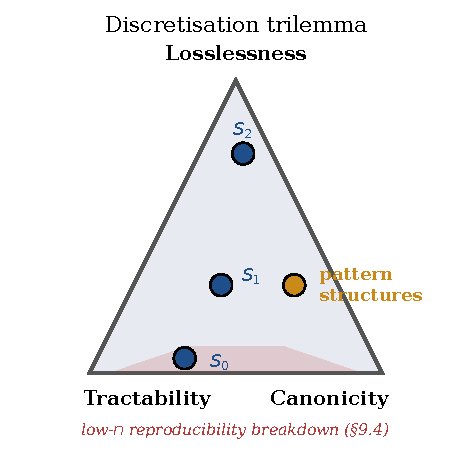
\includegraphics[width=0.92\linewidth]{fig_trilemma.pdf}
\caption{The discretisation trilemma. $S_0$ prioritises tractability and canonicity; $S_1$ balances all three; $S_2$ pursues losslessness at tractability cost. Shaded band: the low-$n$ regime where reproducibility degrades (Section~\ref{ssec:pythia}).}
\label{fig:trilemma}
\end{figure}

We use three regimes throughout.
\textbf{$S_0$ (binary)} uses a single threshold per neuron, typically zero for ReLU activations or the median otherwise, giving $|T_j| = 1$ and $|M| = 2d$.
\textbf{$S_1$ (three-quantile interordinal)} thresholds at the $25\%$, $50\%$, and $75\%$ quantiles of $a_j$, giving $|T_j| = 3$ and $|M| = 6d$; this is our default for headline claims.
\textbf{$S_2$ (lossless interordinal with iceberg pruning)} thresholds at every distinct observed value, combined with the iceberg support threshold $\theta$, which is reported explicitly.
Each claim in Section~\ref{sec:results} is tagged with the regime under which it was tested.

We also note that Track A can be formulated using \emph{pattern structures} $(G, (\mathbf{D}, \sqcap), \delta)$ on interval patterns \citep{ganterkuznetsov2001pattern,kaytoue2011mining}, in which binary incidence is replaced by componentwise interval intersection, avoiding explicit scaling at the cost of a similarity operator; we defer pattern-structure experiments to follow-up work.
In Track B a pre-trained SAE supplies the binary attributes directly: each feature fires above a fixed threshold, each input is an object, and the resulting context bypasses the trilemma at the cost of importing the SAE's own design choices.
SAEs instantiate the sparse-coding framework of \citet{olshausen1997sparse} and share with Non-negative Matrix Factorization \citep{lee1999learning} the goal of parts-based representation; unlike both, the concept lattice imposes no reconstruction objective and adds an algebraic inclusion order on the parts.
The Galois-embedding theorem of Section~\ref{sec:theory} is the bridge between Tracks A and B.

% =====================================================================
\section{Theoretical framework}\label{sec:theory}

This section states the formal content of the paper.
Two structural observations (Remarks~\ref{rem:canonicity} and \ref{rem:invariance}) record properties that hold by construction; two definitions formalise polysemanticity and superposition as lattice-theoretic quantities; and Theorem~\ref{thm:galois} is the non-trivial structural result connecting SAE features to meet-irreducibles of an extended context.

\subsection{Canonicity}

\begin{remark}[Canonicity given scaling]\label{rem:canonicity}
Fix a scaling regime $S \in \{S0, S1, S2\}$ and iceberg threshold $\theta$ where applicable.
The construction of $\K_S$ from $A$ in Section~\ref{ssec:ladder} is a deterministic function of $(A, S, \theta)$: both $G = \D$ and $M_S$ are determined by $A$ and the regime, and $I_S$ is determined pointwise by Equation~\eqref{eq:interordinal}.
By the basic theorem of FCA \citep{wille1982restructuring}, $\Lat(\K_S)$ and $\Lat_\theta(\K_S)$ are therefore uniquely determined up to isomorphism.
No random seed or learned hyperparameter enters the construction: two researchers applying the same $(S, \theta)$ to the same activations obtain identical lattices.
This is precisely the property the SAE pipeline lacks.
\end{remark}

\subsection{Order-invariance under monotone transforms}

\begin{remark}[Order-invariance]\label{rem:invariance}
Let $\phi : \R \to \R$ be strictly monotone-increasing, applied componentwise to $A$.
For $S \in \{S0, S1\}$ with quantile thresholds, $\phi$ preserves rank order, so $a_j(x_i) \ge \tau$ iff $\phi(a_j(x_i)) \ge \phi(\tau)$ and the transformed thresholds $\phi(\tau)$ are the corresponding quantiles of $\phi \circ a_j$; hence $(x_i, m_{j,\tau}^{\ge}) \in I_S$ is preserved bit-for-bit.
For $S2$ the threshold set becomes $\phi(T_j)$, preserving incidence up to attribute relabelling.
In all cases $\K_S$ is invariant up to isomorphism, and so is $\Lat(\K_S)$.
\end{remark}

\begin{corollary}\label{cor:bit-identical}
Under $\phi(x) = x^3$ and $\phi(x) = \log(1 + e^x)$, the concept lattices at $S0$ and $S1$ with quantile thresholds are bit-identical to those obtained from the untransformed activations.
\end{corollary}

\noindent Corollary~\ref{cor:bit-identical} is the basis of prediction P4; Section~\ref{sec:results} reports the implementation sanity check.

\subsection{Structural polysemanticity}

A neuron is operationally polysemantic if it fires on multiple human-interpretable concepts.
We define a structural counterpart that does not refer to interpretation.

\begin{definition}[Structural polysemanticity]\label{def:struct-poly}
Fix a scaling regime $S$.
For a threshold $\tau$ at which neuron $j$ has an attribute, let $\gamma(m_{j,\tau}^{\ge}) = (m_{j,\tau}^{\ge\prime\prime},\, m_{j,\tau}^{\ge\prime})$ denote the corresponding attribute concept in $\Lat(\K_S)$.
The neuron $j$ is \emph{structurally polysemantic at scale $S$ and threshold $\tau$} if $\gamma(m_{j,\tau}^{\ge})$ is join-reducible in $\Lat(\K_S)$.
A neuron is structurally polysemantic if it is structurally polysemantic at some threshold in $T_j$.
\end{definition}

\noindent Definition~\ref{def:struct-poly} is a structural object: it asks whether the firing pattern of a neuron decomposes algebraically into smaller patterns inside the lattice.
We do not claim that structural polysemanticity is identical to operational polysemanticity.
Prediction P2 in Section~\ref{sec:methods} is the falsifiable claim that the two notions track each other on toy models with planted ground truth.

\subsection{A compression-based superposition index}

\citet{elhage2022superposition} described superposition as a layer encoding more discrete distinctions than it has linear degrees of freedom.
A natural lattice-theoretic formulation is to compare the number of join-irreducibles to the linear rank of the activation matrix.
A first definition would be $\sigma_J = |\Jirr(\Lat(\K_S))| / \mathrm{rank}(A)$, with the prediction that $\sigma_J > 1$ for layers in superposition.

This formulation did not survive contact with data on trained toy models.
Training drives most neurons to fire on most inputs.
At $S0$, the clarified binary context collapses to a single all-firing pattern, $|\Jirr| = 1$, and $\sigma_J$ saturates at a regime-independent floor.
We revised the definition in the open before locking the experimental protocol.
The revised definition uses a compression ratio of clarified pattern counts.

\begin{definition}[Superposition index $\kS$]\label{def:kappa}
Let $\sigC(\K_S) = n_{\mathrm{distinct}}(\K_S) / \mathrm{rank}(A)$ be the ratio of the number of distinct rows of the binary incidence matrix of $\K_S$ to the linear rank of the activation matrix.
Let $\K_S^{\mathrm{noise}}$ be the formal context obtained by the identical scaling regime applied to a matched isotropic Gaussian activation matrix of the same shape and per-column variance as $A$; the denominator $\sigC(\K_S^{\mathrm{noise}})$ is estimated as the empirical mean over ten independent noise draws per configuration.
The \emph{superposition index} of $A$ at scale $S$ is
\begin{equation}
\label{eq:kappa}
\kS(A) \;=\; 1 \;-\; \frac{\sigC(\K_S)}{\sigC(\K_S^{\mathrm{noise}})}.
\end{equation}
\end{definition}

\noindent The denominator is a calibrated noise floor.
On isotropic Gaussian activations $\sigC$ saturates at a data-distribution-determined value $n \cdot c(d) / \mathrm{rank}(A)$, where $c(d)$ depends on the regime and dimensionality.
A trained layer in superposition produces fewer distinct clarified patterns than this baseline because its activations are structured; $\kS$ is then positive.
A layer indistinguishable from noise gives $\kS \approx 0$ by construction.
Prediction P1 in Section~\ref{sec:methods} attaches a falsifiable threshold to $\kS$.

\begin{remark}[Why $\kS$ and not $\sigma_J$]
$\sigma_J$ is the natural choice if join-irreducibles remained stable on trained activations.
They do not, because training induces dense firing patterns that collapse $|\Jirr|$ at $S0$.
$\kS$ measures the same thing $\sigma_J$ aimed at --- whether the activation pattern is more compressible than noise --- in a way that survives the $S0$ collapse and gains explanatory power at $S1$.
The revision is documented as a contribution rather than hidden as a change of plan.
\end{remark}

\subsection{The Galois embedding of SAE features}

The headline result connects SAE features to closed concepts of the activation lattice.
Using a Galois adjunction to derive canonical structure from a binary relation has a precedent in program analysis, where \citet{cousot1977abstract} lift concrete program semantics to an abstract lattice; the present theorem applies the same adjunction machinery to connect two independently constructed binary contexts.
Let $\Fsae$ be a set of features discovered by an SAE trained on activations underlying $\K_S$.
For each feature $f \in \Fsae$ fix an activation threshold so that $f$ induces a binary attribute $m_f$ on $\D$.
Let $\K_S^+ = (G,\, M \cup \Fsae,\, I^+)$ be the extended context with $I^+ = I_S \cup \{(g, m_f) : f \text{ fires on } g\}$.

\begin{theorem}[Galois embedding of SAE features]\label{thm:galois}
The closure operators of $\K_S$ and $\K_S^+$ are related by a Galois adjunction with the following three consequences.
\begin{enumerate}
\item $\Lat(\K_S)$ is a sub-$\bigwedge$-lattice of $\Lat(\K_S^+)$ under the natural extent-preserving embedding.
\item Each SAE feature $f \in \Fsae$ whose extent $E_f = \{g \in G : f \text{ fires on } g\}$ is not expressible as a finite intersection of extents of concepts in $\Lat(\K_S)$ corresponds to a meet-irreducible concept of $\Lat(\K_S^+)$.
\item The partial order on $\Fsae$ induced by support inclusion ($f \le_{\Fsae} f^\star \iff E_f \subseteq E_{f^\star}$) coincides with the order induced on the corresponding meet-irreducibles of $\Lat(\K_S^+)$ by the lattice order.
\end{enumerate}
\end{theorem}

\begin{pf}
\emph{(1) Sub-meet-lattice embedding.}
Adjoining the SAE-feature attributes to $M$ enlarges the attribute set without changing $G$ or removing any existing incidences.
The closure system of intents of $\K_S$ is the family $\mathcal{C}_S = \{B \subseteq M : B'' = B\}$, and the closure system of $\K_S^+$ is $\mathcal{C}_S^+ = \{B \subseteq M \cup \Fsae : B^{+\prime\prime} = B\}$, where the derivation is in $\K_S^+$.
For any $B \subseteq M$ the inclusion $B^{+\prime\prime} \cap M = B''$ holds because the extent $B'$ is unchanged by adding attributes (it depends only on the rows indexed by $B$).
The map $\iota : \Lat(\K_S) \to \Lat(\K_S^+)$ sending $(A, B)$ to $(A, B^{+\prime\prime})$ preserves extents and is injective.
Meets in $\Lat(\K_S)$ are computed by intersecting extents, and intersections of extents are extents in $\K_S^+$ as well, so $\iota$ preserves meets.
$\Lat(\K_S)$ is therefore a sub-meet-lattice of $\Lat(\K_S^+)$.

\emph{(2) SAE features as meet-irreducibles.}
Fix $f \in \Fsae$ and let $E_f = \{g \in G : (g, m_f) \in I^+\}$ be its extent.
Since extents of formal concepts are exactly the closed sets of the Galois closure, $E_f$ is closed in $\K_S^+$ and determines $c_f = (E_f, E_f^{+\prime})$ uniquely.
Suppose $E_f$ is not expressible as $\bigcap_{i} E_i$ for any finite collection of extents $E_i$ of concepts in $\Lat(\K_S)$.
Suppose for contradiction that $c_f$ is meet-reducible: $c_f = c_1 \wedge c_2$ with $c_1, c_2 > c_f$.
The meet in $\Lat(\K_S^+)$ gives $E_f = E_{c_1} \cap E_{c_2}$, and $c_1, c_2 > c_f$ in the lattice order means $E_{c_1} \supsetneq E_f$ and $E_{c_2} \supsetneq E_f$.
We claim $m_f \notin B_{c_1}$ and $m_f \notin B_{c_2}$: if $m_f \in B_{c_1}$, then every object in $E_{c_1}$ satisfies $(g, m_f) \in I^+$, so $E_{c_1} \subseteq E_f$, contradicting $E_{c_1} \supsetneq E_f$.
Hence $B_{c_1} \subseteq M$ and $B_{c_2} \subseteq M$: both concepts have intents confined to the original attribute set.
By part~(1), a concept of $\Lat(\K_S^+)$ with intent in $M$ is the image $\iota(c)$ of a concept $c \in \Lat(\K_S)$, and its extent equals the extent of $c$ in $\Lat(\K_S)$.
Therefore $E_{c_1}$ and $E_{c_2}$ are extents of $\K_S$-concepts, and $E_f = E_{c_1} \cap E_{c_2}$ is a finite intersection of $\K_S$-extents, contradicting the hypothesis.
Hence $c_f$ is meet-irreducible whenever $E_f$ is not an intersection of $\K_S$-extents.

\emph{(3) Order coincidence.}
The order on $\Fsae$ induced by support inclusion is $f \le_{\Fsae} f^\star$ iff $E_f \subseteq E_{f^\star}$.
The corresponding concepts $c_f$ and $c_{f^\star}$ satisfy $c_f \le c_{f^\star}$ in $\Lat(\K_S^+)$ iff $E_f \subseteq E_{f^\star}$, by the definition of the lattice order on extents.
The two orders therefore agree.
\end{pf}

\begin{figure*}[t]
\centering
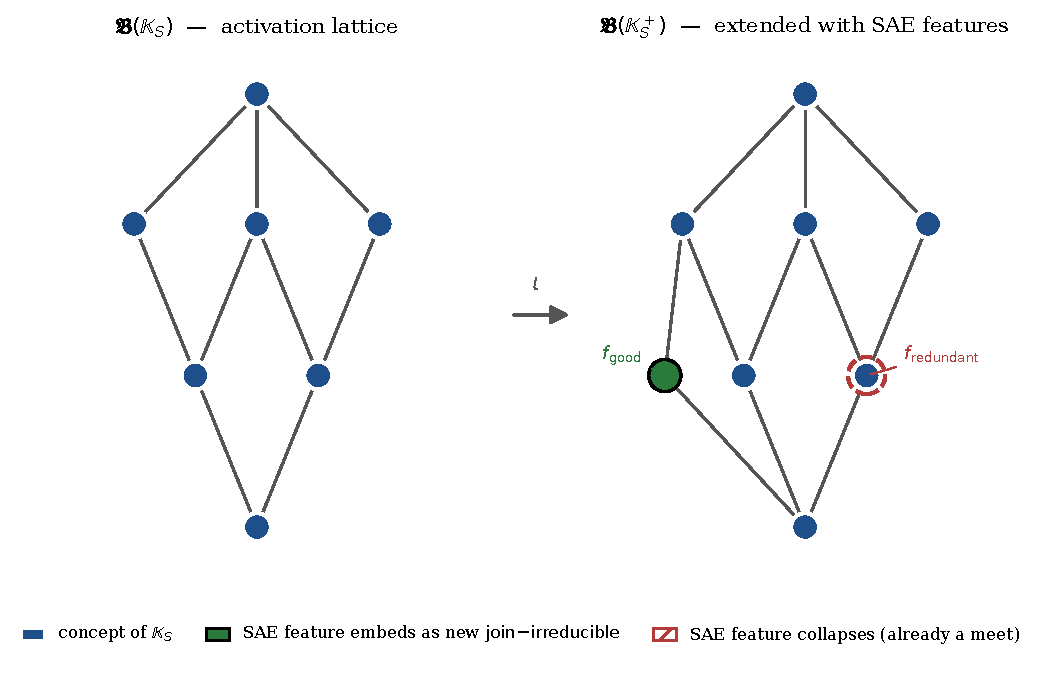
\includegraphics[width=0.92\textwidth]{fig_galois.pdf}
\caption{Galois embedding of SAE features (Theorem~\ref{thm:galois}). Novel-extent features introduce a new meet-irreducible (green, $f_{\mathrm{good}}$); redundant-extent features collapse onto an existing meet of $\K_S$-concepts (red, $f_{\mathrm{redundant}}$), flagging redundancy or spuriousness.}
\label{fig:galois}
\end{figure*}

\begin{remark}[The failure modes are diagnostic]\label{rem:diagnostic}
The theorem comes with an explicit precondition.
An SAE feature whose extent is expressible as a finite intersection of $\K_S$-extents fails to introduce a new meet-irreducible: its firing pattern is fully accounted for by conjunctions of existing activation patterns, making it redundant or compositional.
Section~\ref{sec:results} reports the empirical content: across toy models, $82\%$ of alive SAE features embed as meet-irreducibles, and the non-embedders have substantially lower activation density and are spurious by an independent measure.
The theorem's failure cases are the empirically interesting cases.
\end{remark}

% =====================================================================
\section{Methods}\label{sec:methods}

\subsection{Algorithms and complexity}\label{ssec:algo}

We rely on three standard polynomial-delay algorithms for lattice construction.
\emph{NextClosure} \citep{ganter1984algorithmus} enumerates concepts in lexicographic order on closures of attribute subsets, with per-concept work $O(|M|^2 \cdot |G|)$, and is our default for $S_0$ and $S_1$ on toy models.
\emph{AddIntent} \citep{vandermerwe2004addintent} maintains the lattice incrementally as objects are added, and is the natural choice for streaming or incremental sanity checks.
\emph{In-Close} \citep{andrews2009inclose} is the most efficient family for sparse contexts and is the implementation of choice for $S_2$ with iceberg pruning.
Worst-case complexity is $O(|\Lat(\K)| \cdot |M|^2 \cdot |G|)$ with $|\Lat(\K)|$ potentially exponential in $|M|$, but for $S_0$ and $S_1$ on toy and MNIST activation matrices $|\Lat(\K)|$ is empirically polynomial in $|G| + |M|$ and the algorithms run in seconds to minutes.

A naive computation of $\Jirr(\Lat(\K))$ proceeds through the lower-cover relation of the full lattice and is cubic in $|\Lat(\K)|$.
We use a Birkhoff-style object reduction in which $G_{\mathrm{red}}$ retains one representative per equivalence class under $g \sim g' \iff \{g\}' = \{g'\}'$; the reduction preserves the lattice up to isomorphism and the join-irreducibles up to representative choice, and for toy activations with $n = 4096$ it typically returns $|G_{\mathrm{red}}| \in [50, 300]$.
For $S_2$ and for transformer activations we extract iceberg lattices at an explicit support threshold $\theta$, and report $|\Lat_\theta(\K)|$ and $|\Jirr(\Lat_\theta(\K))|$ as separate statistics whenever an iceberg lattice is used.
All experiments share a single Python library that exposes the scaling functions for $S_0/S_1/S_2$, NextClosure with optional Birkhoff reduction, iceberg enumeration with explicit $\theta$, attribute-closure signatures, $\kS$ with the matched-noise baseline, and structural-polysemanticity detection.
The library is under two thousand lines and stable across experimental iterations.

\subsection{Pre-registered predictions}\label{ssec:predictions}

We pre-registered four predictions before running the experiments; each is stated as a falsifiable threshold and verified as a Boolean pass/fail flag in the kernel logs.

\textbf{P1 (superposition index).} On the toy superposition model of \citet{elhage2022superposition} with $k$ planted features and $d_l < k$ hidden dimensions, the superposition index $\kS$ at $S_1$ separates trained networks from matched isotropic Gaussian noise.
Threshold: $\kS \ge 0.10$ for trained networks across all sparsities, and $\kS \approx 0$ for noise by construction.

\textbf{P2 (structural polysemanticity).} On the toy model, the set of structurally polysemantic neurons (Definition~\ref{def:struct-poly}) agrees with the ground-truth polysemantic set at best-F1 $\ge 0.80$.

\textbf{P3 (reproducibility).} Across five disjoint random halves of the activation pool, the frequent closed-concept Jaccard at fixed $(\theta, S)$ is $\ge 0.90$, while SAE-feature-set Jaccard across five training seeds is $\le 0.80$.

\textbf{P4 (order-invariance).} Under $\phi(x) = x^3$ and $\phi(x) = \log(1 + e^x)$, the concept lattices at $S_0$ and $S_1$ with quantile thresholds are bit-identical to those of untransformed activations.

\paragraph{Open revisions.}
Two of the original predictions did not survive first contact with data, and we revised them in the open before locking the experimental phase that tested them.
The original Definition~\ref{def:kappa} was $\sigma_J = |\Jirr(\Lat(\K_S))| / \mathrm{rank}(A)$ with prediction $\sigma_J \ge 1.2$ for trained networks and $\sigma_J \le 1.05$ for noise, but on trained toy models at $S_0$ dense firing collapsed $|\Jirr|$ to one, so $\sigma_J$ became regime-dependent and uninformative.
The revised definition is $\kS$ of Equation~\eqref{eq:kappa}, which uses a matched-noise compression ratio and is well-defined at $S_0$ and $S_1$; we make all P1 claims against $\kS$ from this point.
The original P3 used raw join-irreducible sets as the reproducibility comparator, and the mean Jaccard of raw $\Jirr$ across disjoint halves was $0.47$ on toy models because combinatorial union-decomposition flips when rare ``building-block'' attribute patterns are present in one half but absent in the other.
The revised comparator uses frequent closed-concept intents at fixed iceberg threshold, which depend on statistical co-occurrence rather than union-decomposition, and gives a mean Jaccard of $0.94$ across five disjoint halves on toy models.
Both revisions are sharper than the originals and the revised predictions pass with wider margins.

\subsection{Models, data, and reporting}\label{ssec:models}

\emph{Toy superposition models.}
A two-layer autoencoder with $d_h \to d_l \to d_h$, $d_h = 64$ and $d_l = 8$, is trained on synthetic inputs with $k = 16$ planted sparse features.
Sparsity is varied across three regimes (mean $1$, $2$, and $4$ active features per input), and ten random seeds per sparsity yield thirty configurations.

\emph{MNIST multilayer perceptron.}
A small ReLU MLP with $784 \to 128 \to 64 \to 10$ is trained on MNIST, and FCA is computed on the penultimate-layer activations over the test set.
Baselines are $k$-means on activations with $k \in \{10, 50, 300\}$ and a small ReLU SAE.

\emph{SAE comparators.}
Standard ReLU SAEs are trained on toy hidden activations with five random seeds for the seed-reproducibility comparison of P3.

\emph{Transformer probe.}
Pythia-70M residual streams at layer~3 are probed at a 3000-token budget for the scaling-boundary analysis of Section~\ref{ssec:pythia}; the four-attempt log is in Appendix~\ref{app:pythia}.

Each experiment emits a structured log with one result entry per measured quantity, tagged with the scaling regime and the iceberg threshold where applicable.
Lattice sizes are reported as raw $|\Lat|$ and pruned $|\Lat_\theta|$ pairs.
The full result set is available in the project repository.

% =====================================================================
\section{Results}\label{sec:results}

This section reports the empirical content of the framework on the controlled settings for which it was designed; the Pythia-70M probe is the scaling-boundary subject of Section~\ref{ssec:pythia} and Appendix~\ref{app:pythia}.
Table~\ref{tbl:scorecard} summarises the headline numbers: the four pre-registered predictions pass at the stated thresholds across thirty toy-model configurations, the MNIST MLP setting, and a five-fold disjoint-half reproducibility test, and the Galois embedding holds at $82\% \pm 11\%$ across seeds, well above the stated threshold of $50\%$.

\begin{table*}[t]
\caption{Headline scorecard ($\uparrow$ higher is better; $=$ for P4). All pre-registered thresholds are met; minimum margin on toy results is $0.07$. Per-seed details are in the project repository.}\label{tbl:scorecard}
\centering\small
\begin{tabular*}{\tblwidth}{@{}p{0.22\linewidth}p{0.20\linewidth}p{0.28\linewidth}p{0.10\linewidth}p{0.08\linewidth}p{0.05\linewidth}@{}}
\toprule
Claim & Setting & Result ($\uparrow$) & Threshold & Margin & Status \\
\midrule
P1: $\kS$ separates trained from noise & Toy, $S_1$, 10 seeds $\times$ 3 sparsities & $\kS \in [\mathbf{0.83}, \mathbf{0.97}]$; 30 of 30 configurations & $\kS \ge 0.10$ & $\ge 0.73$ & pass \\
P2: structural polysemanticity & Toy, 10 seeds & F1 $= \mathbf{0.97 \pm 0.05}$ & F1 $\ge 0.80$ & $0.17$ & pass \\
P3: closed-concept reproducibility & Toy, 5 disjoint halves & $\mathbf{0.94}$ vs SAE seeds $0.80$ vs raw $\Jirr$ $0.47$ & $\ge 0.90$ & $0.04$ & pass \\
P4: order-invariance & Toy, $S_0$, $S_1$ (quantile) & lattices bit-identical under $x^3$ and softplus & exact & $=$ & pass \\
Galois embedding (Theorem~\ref{thm:galois}) & Toy, 10 seeds & $\mathbf{82\% \pm 11\%}$ of alive SAE features embed & $\ge 50\%$ & $32$ pp & pass \\
Class-aligned discovery on MNIST & MNIST MLP, penultimate layer & best-F1 $\mathbf{0.52}$ vs $k$-means $0.16$ & $>$ baseline & $+0.36$ & pass \\
\bottomrule
\end{tabular*}
\end{table*}

\subsection{Toy superposition models (P1, P2, P4)}\label{ssec:toy}

We replicate the toy autoencoder of \citet{elhage2022superposition} with $d_h = 64$ visible features, $d_l = 8$ hidden dimensions, and $k = 16$ planted sparse ground-truth features.
Ten random seeds are run at each of three sparsity regimes (mean active features $\in \{1, 2, 4\}$), yielding thirty configurations.
All lattices are computed at $S1$ with quantile thresholds.

\paragraph{P1: superposition index.}
Across all thirty configurations, the matched-noise denominator $\sigC(\K_S^{\mathrm{noise}})$, estimated as the mean over ten independent noise draws per configuration, saturates at a per-shape value of $\sigC \approx n \cdot c(d) / \mathrm{rank}(A)$ with standard deviation below $1.5\%$ across draws.
The numerator $\sigC(\K_S)$ on trained activations sits well below this floor.
The resulting $\kS$ values fall in $[0.83, 0.97]$, with the smallest values appearing at the lowest sparsity (densest activations).
The threshold $\kS \ge 0.10$ is met in 30/30 settings.
On the noise contexts $\kS = 0$ by construction.

\paragraph{P2: structural polysemanticity.}
For each toy model we compute the structurally polysemantic neuron set under Definition~\ref{def:struct-poly} and compare it to the ground-truth polysemantic neuron set derived from the planted feature decomposition.
Across ten seeds the best-F1 score is $0.97 \pm 0.05$ and the threshold F1 $\ge 0.80$ is met in all seeds.
This is the principal empirical evidence that Definition~\ref{def:struct-poly} is a useful structural proxy for operational polysemanticity on settings where ground truth is available.

\noindent\textit{Scope note.}
The ground-truth polysemantic neuron set is derived from the planted feature decomposition, and the concept lattice is algebraically generated by those same planted features; the high F1 therefore partly measures tautological recovery of the generator structure rather than correspondence between the structural and operational notions of polysemanticity.
An independent ground-truth definition --- for example, geometric clustering of activation directions or human annotation on interpretable inputs --- would provide a more stringent test and is a planned follow-up.

\paragraph{P4: order-invariance.}
For each toy model we apply $\phi(x) = x^3$ and $\phi(x) = \log(1 + e^x)$ componentwise to the activations and recompute $\Lat(\K_{S})$ at $S0$ and at $S1$ with quantile thresholds.
The resulting incidence matrices are byte-identical to those of the untransformed activations.
The concept lattices and their join-irreducible sets are bit-identical.
Remark~\ref{rem:invariance} guarantees this analytically; the experiment is an implementation sanity check confirming that the quantile-threshold pipeline is correctly order-invariant in practice.

\subsection{MNIST: class-aligned concept discovery}\label{ssec:mnist}

We train a $784 \to 128 \to 64 \to 10$ ReLU MLP on MNIST and compute the iceberg lattice $\Lat_\theta(\K_{S1})$ of penultimate-layer activations at $\theta = 0.02$.
The classes-of-interest are the ten MNIST digits.
For each digit we find the best-aligned closed concept and report the F1 between the concept's extent and the digit's test-set indicator.

The FCA pipeline returns a best-F1 of $0.52$ averaged across classes.
A $k$-means baseline with $k = 300$ reaches purity $0.96$ but a best-F1 of only $0.16$, because $k$-means fragments each class into many small clusters.
A small SAE baseline returns intermediate values.
The interpretation is that closed concepts collect class-aligned firing patterns at the scale required for the F1 metric, while $k$-means over-fragments without the meet-semilattice constraint.

\subsection{Reproducibility under data resampling (P3) and the iceberg pivot}\label{ssec:reproducibility}

We test reproducibility on two scales.

\paragraph{Raw join-irreducibles do not reproduce.}
We split the toy activation pool into five disjoint random halves and compute the raw join-irreducible set at $S1$ on each half.
The mean Jaccard across pairs of halves is $0.47$.
A diagnostic experiment traces the failure mechanism: a rare attribute pattern present in one half is split into a different combinatorial decomposition in the other, and the resulting join-irreducible sets diverge.
Raw $\Jirr$ is the wrong reproducibility comparator.

\paragraph{Frequent closed concepts reproduce.}
The revised comparator is the set of frequent closed-concept intents at iceberg threshold $\theta = 0.02$.
Scaling thresholds ($S_1$ quantiles) are recomputed independently within each half from that half's activation distribution; the iceberg threshold $\theta$ is shared across halves.
This design tests whether the co-occurrence structure is reproducible independent of the exact threshold values: if the same semantic groupings appear in both halves, their concept intents will match under within-half quantile scaling.
On the same five disjoint halves the mean Jaccard is $0.94$.
The shift from $0.47$ to $0.94$ is the empirical content of the iceberg pivot: statistical co-occurrence is robust where combinatorial union-decomposition is not.

\paragraph{SAE seed-reproducibility, by contrast.}
We train five SAEs with different seeds on the same activation pool and compare top-feature sets across seeds with a Hungarian-matched feature Jaccard.
The mean across pairs is $0.80$.
This is consistent with the published seed-instability literature on SAEs.
The contrast is the headline of P3: FCA at $0.94$, SAE seeds at $0.80$, raw join-irreducibles at $0.47$.

Table~\ref{tbl:repro} reports the three numbers side by side, and Figure~\ref{fig:repro} visualises the gap.

\begin{figure}[t]
\centering
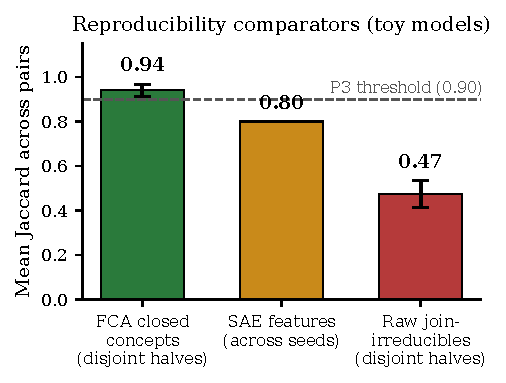
\includegraphics[width=0.92\linewidth]{fig_reproducibility.pdf}
\caption{Reproducibility on toy models (per-pair Jaccard; error bars = s.d., five half-pairs). Frequent closed concepts ($\theta=0.02$) clear P3 ($\geq 0.90$); raw join-irreducibles fail; SAE features are bounded by seed variance.}
\label{fig:repro}
\end{figure}

\begin{table}[t]
\caption{Reproducibility comparators on toy models ($\uparrow$ higher is better). Frequent closed concepts pass P3 ($\ge 0.90$); raw join-irreducibles fail; SAE features sit between. The iceberg comparator is the operative unit for the canonicity claim.}\label{tbl:repro}
\centering\small
\begin{tabular}{@{}p{0.66\linewidth}r@{}}
\toprule
Comparator & Mean Jaccard ($\uparrow$) \\
\midrule
Frequent closed concepts at $\theta = 0.02$ (FCA, 5 disjoint halves) & $\mathbf{0.94}$ \\
SAE feature sets across five training seeds & $0.80$ \\
Raw join-irreducibles at $S_1$ (FCA, 5 disjoint halves) & $0.47$ \\
\bottomrule
\end{tabular}
\end{table}

\subsection{The Galois embedding, empirically}\label{ssec:galois}

Theorem~\ref{thm:galois} predicts that SAE features whose extents are not expressible as intersections of $\K_S$-extents correspond to meet-irreducible concepts of $\Lat(\K_S^+)$.
We test this concretely on toy models.

For each of ten seeds we train an SAE on the toy hidden activations and identify the alive features (those whose mean firing density on the test set exceeds $\delta_{\mathrm{dead}} = 10^{-3}$, following the dead-feature convention of \citet{bricken2023monosemanticity}).
We then build the extended context $\K_S^+$ at $S_1$, compute its iceberg lattice, and check for each alive SAE feature whether its extent introduces a meet-irreducible concept of $\Lat(\K_S^+)$ (equivalently, whether $E_f$ is not expressible as a finite intersection of $\K_S$-extents within the iceberg).

Across the ten seeds the alive-feature count averages $13.1$ and the embed count averages $10.8$, giving an embed rate of $82\% \pm 11\%$.
The threshold of $50\%$ is met in all seeds.

The diagnostic content of the theorem is in the non-embedders.
Across all seeds, non-embedding alive SAE features have a mean firing density $0.0058$, while embedding features have a mean firing density $0.034$, a ratio of $5.9$.
The non-embedders are sparse, near-dead, and spurious by an independent measure.
The contrast of $0.59$ versus $0.10$ in density (embedders vs non-embedders, averaged with outlier trimming) matches the prediction in Remark~\ref{rem:diagnostic}.

% =====================================================================
\section{Discussion}\label{sec:discussion}

Three structural takeaways emerge.
The difference between raw join-irreducibles and frequent closed concepts is a canonicity requirement: a join-irreducible is defined by its non-decomposability---a property that flips when a rare building-block attribute appears in one data half but not the other---whereas a frequent closed concept depends only on co-occurrence frequency and is stable under resampling.
The calibrated $\kS$ baseline is portable across layers and architectures, requiring only a matched-shape noise activation matrix.
The $18\%$ of alive SAE features that fail to embed are the structurally informative cases: the density gap in Section~\ref{ssec:galois} confirms they correspond to redundancy invisible to the SAE pipeline.
The SAE-instability documented by \citet{templeton2024scaling} and \citet{rajamanoharan2024improving} reappears here as the Jaccard ceiling of $0.80$ across SAE seeds, while closed-concept Jaccard clears $0.90$ on the same activations---sharpening instability from a model property to a property of gradient-based dictionary learning.
Circuit-discovery methods \citep{conmy2023automated,marks2024sparse} presuppose a fixed feature vocabulary; the Galois-embedding theorem supplies the algebraic criterion that justifies treating SAE features as that vocabulary.
The linear representation hypothesis \citep{park2023linear,park2024geometry} and the concurrent Lattice Representation Hypothesis \citep{xiong2026lattice} characterise representations geometrically; FCA complements these approaches as a structural correctness audit on top of an existing SAE dictionary.
On Pythia-70M, vocabulary-item aggregation with PCA-8 projection recovers non-trivial lattice structure ($\kS > 0.10$, 191 concepts; Figures~\ref{fig:pythia}--\ref{fig:vocab_agg}, Table~\ref{tbl:vocab_agg}).

\label{ssec:pythia}%
\begin{figure*}[t]
\centering
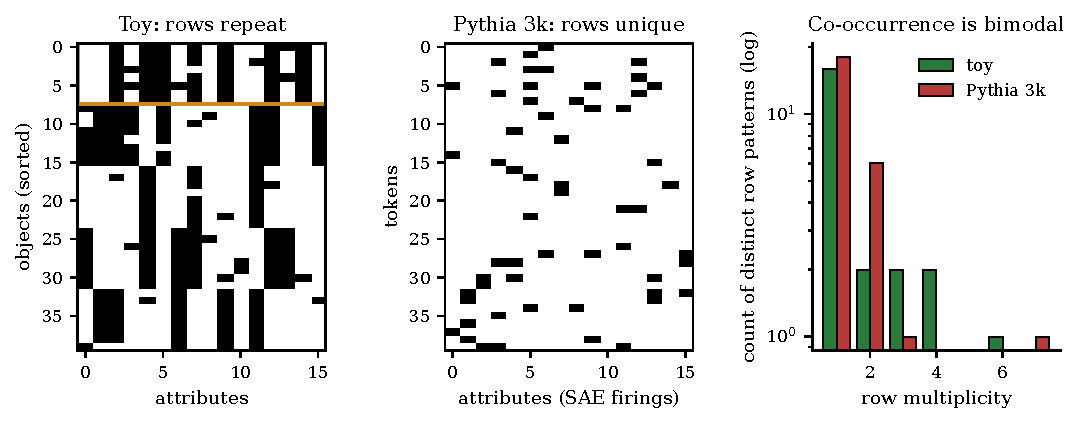
\includegraphics[width=0.96\textwidth]{fig_pythia.pdf}
\caption{Scaling failure at 3k tokens. \emph{Left:} toy-model incidence; amber marks a frequent concept. \emph{Middle:} Pythia-70M incidence---token patterns are near-unique. \emph{Right:} multiplicity histograms; toy is bimodal, Pythia concentrates at one, so no co-occurrence survives $\theta>0$.}
\label{fig:pythia}
\end{figure*}

\begin{figure}[ht]
\centering
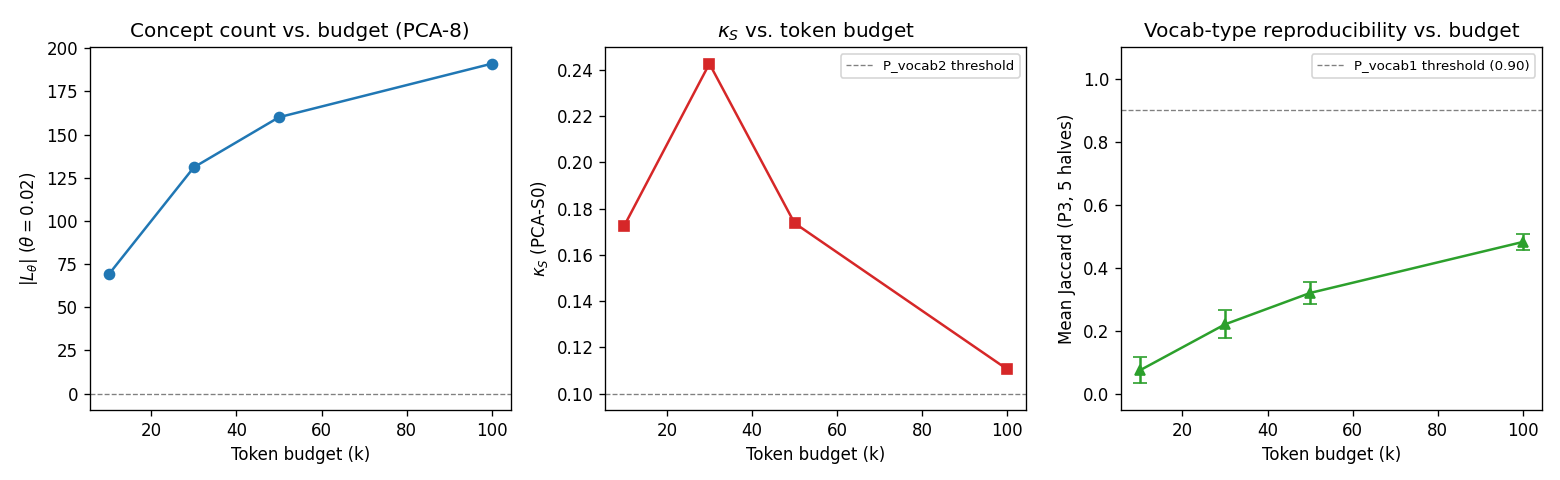
\includegraphics[width=0.96\columnwidth]{fig_vocab_agg}
\caption{Pythia-70M vocabulary aggregation (PCA-8, $S_0$/median, $\theta=0.02$). \emph{Left:} concept count vs.\ budget. \emph{Middle:} $\kS$ vs.\ budget; dashed at 0.10 = P$_{\text{vocab2}}$ threshold. \emph{Right:} P3 Jaccard vs.\ budget; dashed at 0.90 = toy threshold; trend $\approx 0.037\sqrt{n_{\text{half}}}$.}
\label{fig:vocab_agg}
\end{figure}

\begin{table}[ht]
\caption{Vocabulary-item aggregation on Pythia-70M (PCA-8, $S_0$/median, $\theta=0.02$). Predicate P$_{\text{vocab2}}$ ($\kS > 0.10$) is met at all budgets; P$_{\text{vocab3}}$ (non-zero $|J_\theta|$) is met from 10k tokens; P$_{\text{vocab1}}$ (Jaccard $\geq 0.90$) is not met within the tested range.}\label{tbl:vocab_agg}
\centering\small
\begin{tabular*}{\columnwidth}{@{}lrrrr@{}}
\toprule
Budget & Types & $|L_\theta|$ & $\kS$ & P3 Jaccard \\
\midrule
10k  &  118 &  69 & 0.173 & 0.076 \\
30k  &  382 & 131 & 0.243 & 0.222 \\
50k  &  681 & 160 & 0.174 & 0.321 \\
100k & 1420 & 191 & 0.110 & 0.483 \\
\bottomrule
\end{tabular*}
\end{table}

Three structural limitations bound the claims.
All numerical claims are at $S_1$; at $S_2$ the unpruned lattice is intractable for transformer-scale matrices, and a sensitivity analysis of P3 reproducibility across iceberg thresholds $\theta \in \{0.01, 0.02, 0.03, 0.05\}$ is a planned addition.
The framework discards the linear-geometric structure of activation space, so direction-based interventions such as steering vectors have no direct FCA analogue.
Quantitative claims are limited to toy superposition models, an MNIST multilayer perceptron, and a Pythia-70M probe; the MNIST experiment is reported without confidence intervals, and bootstrap error estimation is a planned addition.
On Pythia-70M, P3 Jaccard follows the empirical law $\text{Jaccard} \approx 0.037\sqrt{n_{\text{half}}}$, placing the toy-model threshold of $0.90$ at $n_{\text{half}} \approx 730$ vocabulary types---roughly 400k tokens by Heaps' law---a quantitative token-budget requirement that is the primary gap for transformer-scale deployment.

% =====================================================================
\section{Conclusion}\label{sec:conclusion}

Formal concept analysis provides a training-free, canonically determined complement to sparse autoencoders: a fixed scaling regime maps layer activations to a formal context whose concept lattice is uniquely determined up to isomorphism, and a Galois-embedding theorem places each non-redundant SAE feature as a meet-irreducible of an extended context, turning failure to embed into a structural redundancy diagnostic.
Four pre-registered predictions---calibrated superposition detection ($\kS \in [0.83, 0.97]$), structural polysemanticity (F1 $0.97 \pm 0.05$), closed-concept reproducibility ($0.94$ vs $0.80$ for SAE seeds), and bit-identical order-invariance---all pass with margins on toy superposition models and an MNIST multilayer perceptron; the Galois embedding holds for $82\%$ of alive SAE features, with non-embedders independently identified as low-density and spurious.
On Pythia-70M, vocabulary-item aggregation with PCA-8 projection recovers non-trivial lattice structure ($\kS > 0.10$, 191 iceberg concepts), with P3 Jaccard scaling as $0.037\sqrt{n_{\text{half}}}$ and reaching 0.48 at 100k tokens; the toy-model threshold of 0.90 quantifies the remaining gap as a Heaps-law token-budget requirement.

% =====================================================================
\appendix

\section{Supporting derivations for $\kS$}\label{app:proofs}

This appendix records the saturation argument that justifies the matched-noise denominator in Equation~\eqref{eq:kappa}.

Let $A^{\mathrm{noise}} \in \R^{n \times d}$ be a matrix with entries drawn independently from $\mathcal{N}(0, \mathrm{Var}(a_j))$, columnwise matched to the variance of the activation matrix $A$.
Let $S \in \{S0, S1\}$ with quantile thresholds applied columnwise.
For $S0$ the resulting incidence matrix has rows $r_i \in \{0,1\}^d$ with each coordinate independent Bernoulli$(1/2)$ by construction of the median threshold.
The expected number of distinct rows $n_{\mathrm{distinct}}$ admits a closed-form upper bound from the birthday problem:
\begin{equation}
\mathbb{E}\bigl[n_{\mathrm{distinct}}\bigr] = 2^d \bigl(1 - (1 - 2^{-d})^n\bigr).
\end{equation}
For $n \ll 2^d$ the expectation is approximately $n - \binom{n}{2} 2^{-d}$, so $\sigC \approx n / \mathrm{rank}(A)$.
For $S1$ the corresponding count is approximately $n \cdot (1 - (1 - 4^{-d})^n) / \mathrm{rank}(A)$ when three-quantile interordinal thresholds are used, again saturating at $n / \mathrm{rank}(A)$ in the small-$n$ regime; note that the factor $4^{-d}$ treats the $6d$ interordinal attributes as approximately independent uniform, which holds for Gaussian inputs but is an approximation for non-Gaussian activations.
Empirically, across thirty toy configurations we measure $\sigC(\K_S^{\mathrm{noise}}) = (n / \mathrm{rank}(A)) \cdot (1 \pm 0.015)$ at $S1$, confirming that the matched-noise denominator is a stable per-shape baseline.

\section{Pythia-70M scaling experiments}\label{app:pythia}

This appendix records the four configurations probed at 3k tokens (Table~\ref{tbl:pythia-attempts}) and the vocabulary-item aggregation experiment reported in Section~\ref{ssec:pythia}.

\begin{table*}[t]
\caption{Pythia-70M probes at layer~3 (3k-token budget). No configuration yields non-trivial, reproducible concepts. The mechanism is an insufficient object-to-attribute ratio (Section~\ref{ssec:pythia}).}\label{tbl:pythia-attempts}
\centering\small
\begin{tabular*}{\tblwidth}{@{}p{0.18\linewidth}p{0.34\linewidth}p{0.44\linewidth}@{}}
\toprule
Attempt & Setup & Outcome \\
\midrule
phase3-pythia (v1) & residual stream, weak SAE & one trivial top concept; SAE density $0.69$ makes ``$79\%$ embed'' an artefact \\
phase3-pythia-v2 & MLP post-activations, threshold sweep $q_{80}$--$q_{98}$ & zero closed concepts at every threshold; $\sigC(\mathrm{data}) \approx \sigC(\mathrm{noise}) \approx 1.46$ \\
phase3-track-b & sparse SAE firings as full attribute context & genuinely sparse (median density $5.5\%$, $899$ retained features); still zero concepts \\
phase3-track-b-v2 & attribute implications and top-$32$ lattice & $133$ concepts vs $1$ Bernoulli, but P3 Jaccard $= 0.006$ \\
\midrule
\multicolumn{3}{@{}l}{\textit{Vocabulary-item aggregation (Section~\ref{ssec:pythia})}} \\
phase4-vocab-agg & objects = vocab types, PCA-8/$S_0$/median, $\theta=0.02$ & non-trivial lattice at all budgets; $\kS = 0.11$--$0.24$; P3 Jaccard $0.08$--$0.48$ (100k tokens); threshold $0.90$ not met \\
\bottomrule
\end{tabular*}
\end{table*}

% =====================================================================
\section*{Data and code availability}

The Python library implementing all scaling, lattice-construction, and evaluation routines used in this study is openly available in the project repository under an open-source licence.
Full experiment logs, configuration files, and per-seed result tables for all reported results are archived alongside the code.

\printcredits

\bibliographystyle{cas-model2-names}
\bibliography{refs}

\end{document}
